\chapter[Deployment]{Deployment with Docker} \label{ch:deployment}

\section{Applicability of Containers} \label{applicabilitycontainer}
Containers are becoming an ubiquituous technology. They help increase productivity, operational efficiency and deplyoment velocity while reducing infrastructure cost. As opposed to running several applications on a plain operating system or in a virtual machine, containers are far more flexible because they isolate their dependencies and libraries into their own environment. This also makes it possible to use the same container in a production and development workflow. Containers sit on top of a physical server and its host OS while sharing the OS kernel. They are often compared to virtual machines which need hypervisors in order to virtualize and allocate hardware. Containers on the other hand share resources with the host OS which makes them very lightweight and cost efficient: they are usually only megabytes in size, whereas VMs need gigabytes to run. \autoref{fig:containervsvm} puts containers and VMs into a graphical contrast.

\begin{figure}[H]
    \begin{center}
    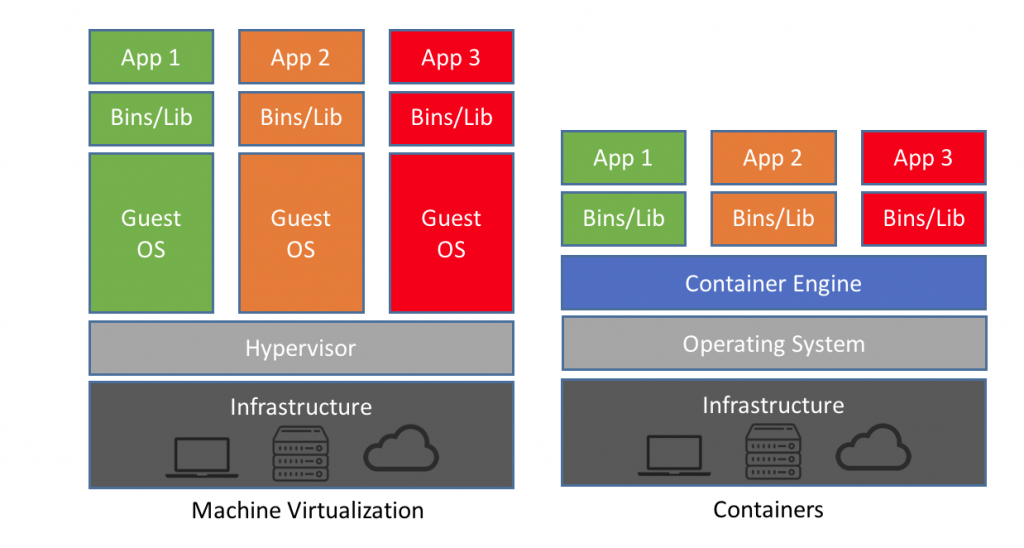
\includegraphics[width=\linewidth]{containervsvm}
    Source: \href{https://blog.netapp.com/wp-content/uploads/2016/03/Screen-Shot-2018-03-20-at-9.24.09-AM-1024x548.png}{blog.netapp.com}
    \end{center}
    \caption{Container vs VMs}
    \label{fig:containervsvm}
\end{figure}
  

\section{Docker}
Docker, the most widely used application-level containerization technology advertises itself as a platform to "Build, Ship, and Run Any App, Anywhere" and is used within the project. It provides the benefits described in \autoref{applicabilitycontainer} and its community offers a wide variety of pre-built container images on its "Hub" registry. Popular offical images include PostgreSQL, NGINX, Django and Apache whereas custom images are often built on top of these. An image is defined with a "Dockerfile" that contains all the commands needed to assemble it. Docker "compose" files are a common way of defining and running multi-container applications. For example it is possible to define a webservice and frontend application which communicate with each other. In addition to Docker, Docker Swarm is used for cluster management, deployment and load balancing.

\section{Microservices}
The main components of the project are separated into three microservices: \textbf{Frontend}, \textbf{Backend} and \textbf{Database}. The source code along with the Dockerfile of each service can be found in the respective identically named folder. Each microservice is encapsulated in its own container and the production-ready composition of all can be found in the file "hv-prod.yml" which is depicted in \autoref{dockerprod}. A slightly different development environment is defined in "hv-dev.yml".

\subsection{Frontend}
The frontend utilizes a multi-staged environment in which the code is first built within a node image and the resulting output copied into an nginx image. Multi-stage builds allows the creation of multiple intermediary images from the same Dockerfile. The main benefit being that the application's build-dependencies are not included in the final image, thus making it smaller and more portable. 

\subsection{Backend}
As the backend was already existing, changes had to be made in order to integrate it into a Docker workflow. The source code included in "Deliverable 2" contains those files, were changes were necessary, not however the full source code of the backend. Namely, the requirements.txt settings.py files had to be adapted. Additionally, a Dockerfile to build the backend image had to be created. The settings.py file had to be changed in a way that allowed for referencing other containers by their hostname and to use a secret file provided by Docker Swarm containing the various password for the system. These changes are annotated inline.

\subsection{Database}
In the database folder a Dockerfile is included for bootstrapping a PostgreSQL database. Additionally, the folder contains an init.sql file which is used for initially creating tables and users. In the Dockerfile it is defined that init.sql is to be copied into /docker-entrypoint-initdb.d/10-init.sql of the PostgreSQL image. According to its documentation, any .sql or .sh file is executed where as the prefixed number dictates the priority. E.g 10 runs before 20.

\subsection{Alpine Linux}
In order to keep the image size small, the especially lightweight linux distribution "Alpine Linux" was chosen as the base OS for every container. Its size has made it a popular choice amongst Docker users: as opposed to Ubuntu which usually needs several hundred MB, Apline's base system size is only 4 to 5 MB big.

\subsection{Reverse Proxy}

\section{Deployment}
DigitalOcean was chosen as a IaaS platform

Additionally, the YAML files in the root folder define the complete docker environment needed to bootstrap the whole application with all its microservices. The hv-dev.yml file defines a development environment which does not include a reverse proxy, thus being a little bit more portable. 

The hv-prod.yml is used in tandem with the traefik.yml file. The first contains pretty much the same data as the dev file with the addition of so-called "labels". These labels are retrieved by the reverse-proxy container "traefik", which is defined in the traefik.yml file. By using labels traefik knows which containers to route to when a certain domain or subdomain is accessed. All files mentioned are also annotated to make it a little easier to understand what is going on.

As the main part of the project was to create a single page application, the most interesting code to look at is located in the frontend folder.

Interesting parts to look at:
- frontend
    - contains single page application - main part of project
    - Dockerfile: contains image definitions for building frontend and serving with webserver
- backend
    - Dockerfile: contains image definitions for building backend
    - settings.py: configuration for django made compatible with docker
- hv-dev.yml
    - defines how all services work together in a dev environment
- hv-prod.yml
    - defines how all services work together in a production environment with a reverse proxy
- traefik.yml
    - defines reverse-proxy image with additional key value store for storing and reusing SSL certificates
- traefik-config.toml
    - configures traefik service in detail

Disclaimer: The contents of this file are discussed in the project report in far greater detail. The intention of this file is to give a brief overview of the technical parts of the project and to serve as a navigation guide for the source code. 
